\documentclass[11pt, oneside]{article}   	% use "amsart" instead of "article" for AMSLaTeX format
\usepackage{geometry}                		% See geometry.pdf to learn the layout options. There are lots.
\geometry{letterpaper}                   		% ... or a4paper or a5paper or ... 
%\geometry{landscape}                		% Activate for rotated page geometry
%\usepackage[parfill]{parskip}    		% Activate to begin paragraphs with an empty line rather than an indent
\usepackage{graphicx}				% Use pdf, png, jpg, or eps§ with pdflatex; use eps in DVI mode
								% TeX will automatically convert eps --> pdf in pdflatex		
\newcommand{\vx}{\vec{x}}
\newcommand{\vxj}{\vec{x}_{j}}
\newcommand{\vxi}{\vec{x}_{i}}
\newcommand{\bx}{{\bf{X}}}
\newcommand{\vy}{\vec{y}}
\newcommand{\yj}{y_{j}}
\newcommand{\yi}{y_{i}}
\newcommand{\vb}{\vec{\beta}}
\newcommand{\va}{\vec{\alpha}}
\newcommand{\px}{\mathcal{P}(\vec{x};\vec{\beta)}}
\newcommand{\pxj}{\mathcal{P}(\vec{x}_{j};\vec{\beta})}
\newcommand{\dpx}{\mathcal{P}'(\vec{x};\vec{\beta})}
\newcommand{\dpxj}{\mathcal{P}'(\vec{x}_{j};\vec{\beta})}
\newcommand{\until} {\mathcal{U} }
\newcommand{\glmnet} {\tt glmnet}


\usepackage{amssymb}
\usepackage{amsmath}
%SetFonts

%SetFonts


\title{Notes on MVA}
\author{Thomas Gadfort}
\date{\today}							% Activate to display a given date or no date

\begin{document}
\maketitle


\section{Classification}

A classification algorithm (classifier) is represented by a decision function $f(\vx) : V \rightarrow~\{-1,1\}$~such that $f(\vx) = 1$~if the classifier assigns $\vx$~to the first class, and $f(\vx) = -1$~if the classifier assigns $\vx$~to the second class.

\section{Linear Model}
A model with a formula of the form
\begin{equation}
\yj = \sigma(\va\cdot\vxj + \alpha_{0})
\end{equation}
where $\yj$ is the $j^{\rm{th}}$~entry of the dependent variable, $\vxj$~is the $j^{\rm{th}}$~set of features (variables), and $\va$~are the fit parameters ($\alpha_{0}$~is a constant offset). The fit parameters are determined by maximizing the following objective function or loss function,~$L$. That is, determine the set of $\va$~that satisfy~$\partial L / \partial \va = 0$.
\begin{equation}
L = [y - (\vec{\alpha}\cdot\vec{x} + \alpha_{0})]^{2}
\end{equation}




\section{Generalized Linear Model}


\subsection{Solution to Logistic Regression}

The maximum likelihood (L) solution for $\va$~maximizes the following product over all training data,

\begin{equation}
L(\vy~|~\bx ; \va)  \equiv \left[ \prod_{j}^{N} \pxj \right] \times \left[ \prod_{j}^{N} (1-\pxj) \right]
\end{equation}

That is, the product of all observations assuming a true event, i.e., $\pxj$~for event $j$~and the product of all observations assuming a false event, i.e., $1-\pxj$. In this equation, $\vy$~is the vector of outcomes, $\bx$~is the matrix of features (i.e., $\vxj$~for outcome each outcome $\yj$).

Mathematically it is simpler to maximize the log-likelihood function (LL or $\mathcal{L} \equiv \mathcal{L}(\vy~|~\bx;\va)$) given as,
\begin{equation}
\mathcal{L}(\vy~|~\bx;\va) = \left[ \sum_{j}^{N} \log (\pxj) \right] \times \left[ \sum_{j}^{N} \log(1 - \pxj) \right]
\end{equation}

The solution for the model parameters is found by solving $d\mathcal{L}/d{\vec{\alpha}} = 0$. The partial derivative or gradient is defined as,
\begin{equation}
\frac{ \partial \mathcal{L} }{ \partial \vec{\alpha} } = \nabla_{\vec{\alpha}} \mathcal{L} = \sum_{j}^{N} \frac{1}{\pxj} \dpxj - \sum_{j}^{N} \frac{1}{1-\px} \dpxj
\end{equation}

Using $\dpx = \px(1-\px)$, we find,
\begin{eqnarray*}
\nabla_{\va} \mathcal{L}	&=& \sum_{j}^{N} \frac{1}{\pxj} \pxj(1-\pxj) - \sum_{j}^{N} \frac{1}{1-\pxj} \pxj(1-\pxj) \nonumber \\
							&=& \sum_{j}^{N} (1-\px) - \sum_{j}^{N} \px
\end{eqnarray*}

Combining the two sums representing $\yj=1$~and $\yj=0$, and inserting ($\yj - \yj$) into the numerator yields,
\begin{eqnarray*}
\nabla_{\va} \mathcal{L} &=&  \sum_{j}^{N} \yj(1-\px) - (1-\yj)\px
\end{eqnarray*}

\section{Derivation of Logistic Regression}
We assume that the case of interest (or "true") is coded to $\bf{1}$, and the alternative case (or "false") is coded to $\bf{0}$.

The logistic regression model assumes that the log-odds of an observation $y$ can be expressed as a linear function of the input variables $\vx$. That is,
\begin{equation}
\log \left[ \frac{\px}{1-\px} \right] = \sum_{i}^{N} \alpha_{i}x_{i} = \va \cdot \vx
\end{equation}
where $\px$~is the probability of observing $\yj$~given $\vxj$~and $\va$. The left-hand-side of the equation is known as the $\it{logit}$~of $\px$. Exponentiating each side yields,
\begin{eqnarray}
	\frac{\px}{1-\px}	&=& \rm{exp} \left[ {\sum_{i}^{N} \alpha_{i}x_{i}} \right] \\
				&=& \prod_{i}^{N} \rm{exp}(\alpha_{i}x_{i})
\end{eqnarray}
Inverting the $\it{logit}$~equation gives,
\begin{equation}
\px = \left[ \frac{e^{z}}{1 + e^{z}} \right]
\end{equation}
where,
\begin{equation}
z = \sum_{i}^{N} \alpha_{i}x_{i} = \vec{\alpha}\cdot\vec{x}
\end{equation}


\subsection{Derivation of $\mathcal{P}'(z)$}
 $\mathcal{P}'(z)$~is defined as,
\begin{equation}
\mathcal{P}(\vec{x}) = \left[ \frac{e^{z}}{1 + e^{z}} \right]
\end{equation}

Taking the derivative yields,
\begin{eqnarray}
\mathcal{P}'(\vec{x})	&=& \left[ \frac{e^{z}}{1 + e^{z}} \right] +  \left[ \frac{-(e^{z})^{2}}{(1 + e^{z})^{2}} \right] \\
				&=& \frac{e^{z}}{(1 + e^{z})^{2}} \\
				&=& \frac{e^{z}}{(1 + e^{z})} \cdot \frac{1}{(1 + e^{z})} \\
				&=& [\mathcal{P}(z)][1-\mathcal{P}(z)]
\end{eqnarray}


\section{{\glmnet}: Lasso and Elastic-Net Regularized Generalized Linear Models}

{\glmnet}~is a package that fits a generalized linear model via penalized maximum likelihood. In this model, the following is minimized loss function,

\begin{equation}
L = \frac{1}{N} \sum_{i}^{N} \omega_{i} \times \ell(\yi; \vb ; \vxi) + \lambda \left[ \frac{1}{2}(1 - \alpha) || \vb ||_{2}^{2} + \alpha || \vb ||_{1} \right]
\end{equation}

where $\omega_{i}$~is the weight given to event $i$, $\vb$~are the fit parameters, $\ell(y,\eta)$~is the negative log-likelihood contribution for event $i$~and $\alpha$~is the elastic-net penalty that bridges the gap between the {\tt lasso}~technique where $\alpha=1$~and the {\tt ridge}~technique where $\alpha=0$. The tuning parameter $\lambda$~controls the overall strength of the penalty.

\subsection{Gaussian Family}

The gaussian family is identical the linear regression with the additional penalty term. The objective function for this family is then written as

\begin{equation}
L = - \left[ \frac{1}{N} \sum_{i}^{N} (\yi - (\vb \cdot \vxi))^{2}  \right] + \lambda \left[ \frac{1}{2}(1 - \alpha) || \vb ||_{2}^{2} + \alpha || \vb ||_{1} \right]
\end{equation}


\subsection{Binomial Family}

The response variable for the binomial model takes the form

\begin{equation}
\px = \frac{e^{\vb \cdot \vx}}{1 + e^{\vb \cdot \vx}}
\end{equation}

The objective function for this family is then written as

\begin{equation}
L = - \left[ \frac{1}{N} \sum_{i}^{N} \yi (\vb \cdot \vxi) - \log (1 + e^{\vb \cdot \vxi}) \right] + \lambda \left[ \frac{1}{2}(1 - \alpha) || \vb ||_{2}^{2} + \alpha || \vb ||_{1} \right]
\end{equation}

\subsection{Poisson Family}

The objective function for this family is then written as

\begin{equation}
L = - \left[ \frac{1}{N} \sum_{i}^{N} \yi (\vb \cdot \vxi) - e^{\vb \cdot \vxi} \right] + \lambda \left[ \frac{1}{2}(1 - \alpha) || \vb ||_{2}^{2} + \alpha || \vb ||_{1} \right]
\end{equation}

\subsection{Cox Model}

The Cox proportional hazards model is commonly used for the study of the relationship between predictor variables and survival time. In the usual survival analysis framework, we have data of the form ($y_{1}, x_{1}, \delta_{1}$), ..., ($y_{1}, x_{1}, \delta_{1}$) where $\yi$, the observed time, is a time of failure if $\delta_{i}$~is 1 or right-censoring if $\delta_{i}$~is 0. We also let $t_{1} < t_{2} < . . . < t_{m}$~be the increasing list of unique failure times, and $j(i)$~denote the index of the observation failing at time $t_{i}$.

The Cox model assumes a semi-parametric form for the hazard
\begin{equation}
h_{i}(t) = h_{0}(t) e^{\vb \cdot \vxi}
\end{equation}

where $h_{i}(t)$~is the hazard for patient $i$~at time $t$, $h_{0}(t)$~is a shared baseline hazard, and $\vb$~is a fixed vector of length $p$. In the classic setting $n \ge p$, inference is made via the partial likelihood,

\begin{equation}
L(\vb) = \prod_{i}^{m} \frac{e^{\vb \cdot \vxi}}{\sum_{j}^{R_{i}} e^{\vb \cdot \vxj}}
\end{equation}

where $R_{i}$~is the set of indices $j$~with $y_{j} \ge t_{i}$ (i.e., those at risk at time $t_{i}$).





\section{{\tt ranger}: A Fast Implementation of Random Forests}

Use this...

\section{{\tt gbm}: Generalized Boosted Regression Models}

\section{{\tt earth}: Multivariate Adaptive Regression Splines (MARS)}

MARS builds models with an estimator of the form

\begin{equation}
f(\vx) = \sum_{i}^{K} c_{i} B_{i}(\vx)
\end{equation}

where $B_{i}(\vx)$~is the $i^{\rm{th}}$~basis function of the input features $\vx$~and $c_{i}$~is the weight for that basis function. Each basis function takes one of the following three forms:
\begin{itemize}
\item Constant 1
\item A hinge function. A hinge function has the form $\max(0, x - c)$~or $\max(0, c - x)$.
\item Product of hinge functions.
\end{itemize}


\section{{\tt RSNNS}: Neural Networks in R using the Stuttgart Neural Network Simulator (SNNS)}

Doesn't work with MLR yet.

\section{Support Vector Machines (SVM)}

Start with a set of $N$~points for the feature set $\vx$ for each outcomes $\yj$. The goal is to find a hyperplane that separates (maximally divides) the points belonging to $\yj=1$~(TRUE)~and $\yj=-1$~(FALSE). Generally, a hyperplane is defined as
\begin{equation}
\vec{w} \cdot \vx - b = 0
\end{equation}
where $w$~is the normal vector and the parameter $b/||\vec{w}||$~is the offset from the origin along the $w$~vector.

Since we can arbitrary scale parameters $\vec{w},b$~defining fixed hyperplane $\pi$, we can choose $\vec{w},b$ such that $||\vec{w}|| = 1$. Note that this pair of parameters is unique for any hyperplane. The distance $\rho(\vx,\pi)$~between a $\vx$~and a hyperplane $\pi(\vec{w},b)$~can be calculated according to the following equation:
\begin{equation}
\rho(\vx,\pi)= \frac{\langle \vec{w},\vx \rangle}{||\vec{w}||}
\end{equation}

Two classes are called linearly separable if there exists at least one hyperplane that separates them. If hyperplane $\rho(\vx,\pi)$~separates classes $C_{1}$~and $C_{2}$, then decision function
\begin{eqnarray}
f(\vx) = {\rm{sign}}\{\langle \vec{w},\vx \rangle + b\}	&= 1 & {\rm{if}}~ \langle \vec{w},\vx \rangle + b > 0 \\
										&= -1 & {\rm{if}}~ \langle \vec{w},\vx \rangle + b < 0
\end{eqnarray}
gives us a classifier that correctly classifies all vectors from $C_{1}$~and $C_{2}$.

For a hyperplane $\pi$~separating classes $C_{1}$~and $C_{2}$, its margin $m(\pi, C_{1}, C_{2})$~is defined as the distance between $\pi$~and class $C_{1}$, plus the distance between $\pi$~and class $C_{2}$.
\begin{equation}
m(\pi, C_{1}, C_{2}) = \rho(\pi, C_{1}) + \rho(\pi, C_{2})
\end{equation}

The objective function for an SVM is given by
\begin{eqnarray}
L = \frac{1}{2} \sum_{k}^{n} w_{k}^{2} + C \sum_{j}^{l} \chi_{j},~~{\rm{such~that}} \\
\yj \left( \sum_{k}^{n} w_{k} x_{jk} + b \right) \ge 1 - \chi_{j} \\
\chi_{j} \ge 0
\end{eqnarray}

This is known as the soft max SVM solution with tunable parameter $C$.

\begin{figure}[htbp]
\begin{center}
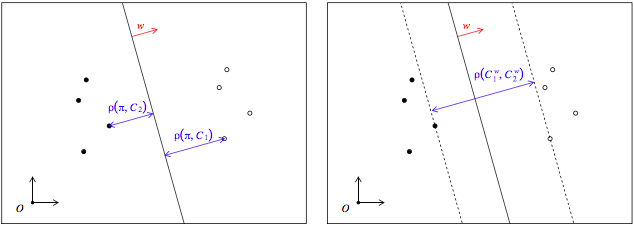
\includegraphics[]{svm/svmDist.png}
\caption{default}
\label{default}
\end{center}
\end{figure}

\begin{figure}[htbp]
\begin{center}
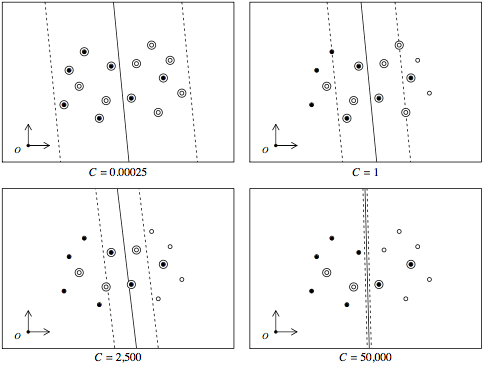
\includegraphics[]{svm/svmC.png}
\caption{default}
\label{default}
\end{center}
\end{figure}



The goal of the SVM is to minimize $||\vec{w}||$~subject to the criterion,
\begin{equation}
\yj (\vec{w} \cdot \vxj - b) \ge 1
\end{equation}

\subsection{Kernals}
Kernels are the idea of summing functions that imitate similarity (induce a positive-definite encoding of nearness) and support vector machines are the idea of solving a clever dual problem to maximize a quantity called margin. We can now restate what a support vector machine is: it is a method for picking data weights so that the modeling function for a given kernel has a maximum margin.



\end{document}  